\documentclass[11pt,a5paper]{article}

\usepackage[T1]{fontenc}
\usepackage[utf8]{inputenc}
\usepackage{lmodern, microtype}
\usepackage[estonian]{babel}
\usepackage{siunitx}
\sisetup{inter-unit-product=\ensuremath{{}\cdot{}}, per-mode=fraction, exponent-product=\cdot, output-decimal-marker={,}}
\usepackage{graphicx}
\usepackage{wrapfig}
\usepackage{adjustbox}
\usepackage{tikz}
\usetikzlibrary{arrows.meta, patterns, patterns.meta}
\usepackage{pgfplots}
\usepackage[european]{circuitikz}
\tikzset{component/.style={draw,thick,circle,fill=white,minimum size=0.75cm,inner sep=0pt}}
\usepackage{amsmath,amssymb}
\usepackage{amsfonts}
\usepackage[hidelinks]{hyperref}
\usepackage{csquotes}
\usepackage{caption}
\usepackage{enumitem}
\topmargin=-3.0cm \textheight=19cm \textwidth=12.9cm
\oddsidemargin=-1.5cm  \evensidemargin=-1.5cm
\setlength{\parindent}{0pt} \setlength{\parskip}{6pt} \sloppy
\sloppy \relpenalty=10000 \binoppenalty=10000
\pagestyle{empty}
\usepackage{derivative}

\newcommand{\numb}[1]{\vspace{5pt}\textbf{\large #1}}
\newcommand{\nimi}[1]{(\textsl{\small \uppercase{#1}})}
\newcommand{\punktid}[1]{(\emph{#1~p.})}
\newcounter{ylesanne}
\newcommand{\yl}[1]{\addtocounter{ylesanne}{1}\numb{\theylesanne.} \nimi{#1} \newblock{}}
% \newcommand{\autor}[1]{}% Kasuta võistluse ajal
\newcommand{\autor}[1]{\emph{Autor: #1}}% Kasuta kui vaja autorit

\begin{document}

\begin{center}
  \textbf{\Large Eesti koolinoorte 71. füüsikaolümpiaad} \par
  \emph{6. aprill 2024. a. Lõppvoor \\Gümnaasiumi ülesannete lahendused (10.--12. klass)}
\end{center}

\yl{Kelgumägi}
\punktid{6} \autor{Hans Daniel Kaimre}
Lähendame Sandrat mäest alla kelgutades klotsina kaldpinnal (vt joonist). Sandrale mõjub raskusjõud $F_r=mg$, mille kaldpinna suunaline komponent on $mg\sin\alpha$ ning pinnanormaali suunaline komponent on $mg\cos\alpha$. Pinnanormaali suunaline komponent on võrdne toereaktsiooniga, st $N=mg\cos\alpha$. Kelgule mõjuv liughõõrdejõud on võrdeline toereaktsiooni ja jõõrdeteguriga: $F_h=\mu N=\mu mg\cos\alpha$. Seega Sandrat nõlval pidurdav jõud on $F_p = mg(\mu \cos\alpha - \sin\alpha)$, kust kiirendus $a=F_p/m=g(\mu \cos\alpha - \sin\alpha)$.
\begin{center}
\includegraphics[width=0.45\textwidth]{keha_slope.png}
\end{center}
Ühtlase kiirendusega liikumise kirjeldamiseks kehtib valem $s=(v^2-v_0^2)/2a$, kus $s$ on nihe, $v$ keha lõppkiirus, $v_0$ keha algkiirus ning $a$ kehale mõjuv kiirendus. Piirjuhul jääb Sandra nõlva lõppu jõudes seisma, st $v=0$, kiirendus $a=-g(\mu \cos\alpha - \sin\alpha)$ (miinusmärgiga, kuna kiirendus on keha liikumise suunaga võrreldes vastassuunas) ning nihke leiame trigonomeetriast: $s=h/\sin\alpha$. Seega
\[
  \frac{h}{\sin\alpha} = \frac{-v_0^2}{-2g(\mu \cos\alpha - \sin\alpha)}.
\]
Millest
\begin{align*}
  v_0 &= \sqrt{\frac{2hg(\mu \cos\alpha - \sin\alpha)}{\sin\alpha}}\\
  &= \sqrt{\frac{2\cdot\SI{6}{\m}\cdot \SI{9.8}{\m\per\s\squared}  \cdot (0.3\cdot \cos \SI{15}{\degree}  - \sin\SI{15}{\degree})}{\sin\SI{15}{\degree}}} = \SI{3.8}{\m\per\s}.
\end{align*}

\newpage
\yl{Ragulka}
\punktid{6} \autor{Taavi Pungas}
Kivike on raske ja väike, seega õhutakistusega pole heas lähenduses vaja arvestada. See võimaldab meil kasutada energia jäävuse seadust. Lähendame ragulka kummi kui lineaarse elastsusega materjali, st kehtib Hooke'i seadus. Kivikese lennu haripunktis on elastsusjõu potentsiaalne energia ragulka kummi venitamisel täpselt teisenenud raskusjõu potentsiaalseks energiaks:
\[
  \frac{kx^2}{2} = mgh.
\]
Jagades läbi selle valemi teise ja esimese katse jaoks, saame
\[
  \frac{x_2^2}{x_1^2} = \frac{h_2}{h_1},
\]
seega
\[
  x_2 = x_1 \cdot \sqrt{\frac{h_2}{h_1}} = \SI{3}{\cm} \cdot \sqrt{\frac{1}{1- \frac{1}{4}}} \approx \SI{3,5}{\cm}.
\]

\yl{Leedid}
\punktid{8} \autor{Sandra Schumann}
Patareid lühistada ei tohi, seega dioode otse patarei külge ühendada ei tohi. Järelikult peavad dioodid olema mingis kombinatsioonis jadamisi takistitega. Tahame, et dioodide põlemise korral läbiks neid voolutugevus $\SI{20}{\mA}$. Ilmselt peab vähemalt selline voolutugevus läbima ka vähemalt ühte takistit. Kui see voolutugevus läbib \SI{300}{\ohm} takistit, siis sellel on pingelang $\SI{6}{\V}$, läbides \SI{360}{\ohm} takistit oleks pinge \SI{7.2}{\V}.

Märkame nüüd, et dioodide põlemiseks vajalike päripingete ja soovitud voolutugevustel olevate patareide pingelangude summad saavad võrduda patarei pingega kahel juhul: punane dioodi jadamisi \SI{360}{\ohm} takisti ja patareiga ning sinine diood jadamisi \SI{300}{\ohm} takisti ja patareiga.

Rakendades tingimust, et vastavat värvi lülitit vajutades peab minema põlema vastavat värvi diood, saame kaks võimalikku skeemi:
\begin{center}
  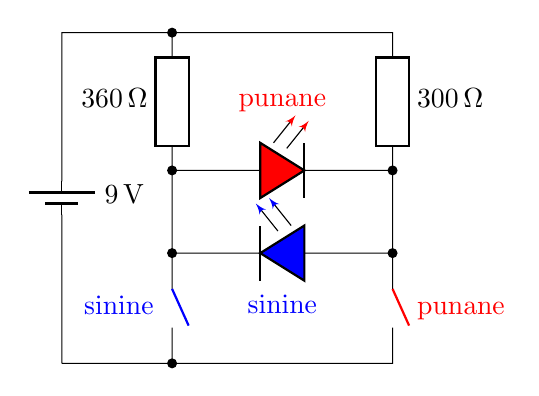
\begin{tikzpicture}[scale=0.7]
    \draw (0,0) to[battery1, l_=\SI{9}{\V}, invert] (0,6) to[short] (2,6) to[short] (6,6) to[R=\SI{300}{\ohm}] (6,3.5) to[short, *-*] (6,2) to[nos, color=red, l=punane, red] (6,0) to[short, -*] (2,0) -- (0,0);
    \draw (2,6) to[R, l_=\SI{360}{\ohm}, *-] (2,3.5) to[short, *-*] (2,2) to[nos, color=blue, l_=sinine, blue] (2,0);

    \draw (2,3.5) to[led, l=punane, fill=red, red] (6,3.5);
    \draw (2,2) to[led, l_=sinine, invert, fill=blue, blue] (6,2);
  \end{tikzpicture}
  \hspace{-1cm}
  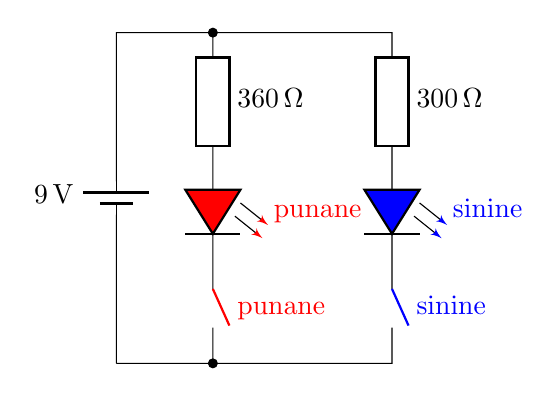
\begin{tikzpicture}[scale=0.7]
    \draw (1,0) to[battery1, l=\SI{9}{\V}, invert] (1,6) to[short] (2,6) to[short] (6,6) to[R=\SI{300}{\ohm}] (6,3.5) to[led, l=sinine, fill=blue, blue] (6,2) to[nos, color=blue, l=sinine, blue] (6,0) to[short, -*] (2.75,0) -- (1,0);
    \draw (2.75,6) to[R, l=\SI{360}{\ohm}, *-] (2.75,3.5) to[led, l=punane, fill=red, red] (2.75,2) to[nos, color=red, l=punane, red] (2.75,0);
  \end{tikzpicture}
\end{center}

Meil peab veel kehtima ka tingimus, et mõlema lüliti vajutamisel ei põleks kumbki diood. See on tõene ainult vasakpoolse skeemiga. Seega just see skeem tulebki koostada.

\yl{PILJARD}
\punktid{8} \autor{Richard Luhtaru}\par
\osa Olgu piljardikuuli kiirus enne põrget $v_0$ ja pärast põrget $v_1$. Olgu $x$-telg servaga paralleelne ja $y$-telg servaga risti. Kuna serv mõjutab kuuli ainult $y$-sihis, siis kuuli $x$-suunaline kiirus ei muutu põrke jooksul. Seega
\begin{equation*}
    v_x = v_0\sin\ang{45} = v_1\sin\ang{60} \implies \frac{v_1}{v_0} = \frac{\sin\ang{45}}{\sin\ang{60}}.
\end{equation*}
Kuna kuuli kineetiline energia on $E = \frac{1}{2}mv^2$, siis
\begin{equation*}
    \frac{E_1}{E_0} = \frac{\frac{1}{2}mv_1^2}{\frac{1}{2}mv_0^2} = \frac{v_1^2}{v_0^2} = \frac{\sin^2\ang{45}}{\sin^2\ang{60}} = \left(\frac{\sqrt{2}/2}{\sqrt{3}/2}\right)^2 = \frac{2}{3},
\end{equation*}
seega põrke käigus läks kaduma umbes $33\%$ palli energiast.

\osa Newtoni teisest seadusest
\begin{equation*}
    F = ma = m\frac{\Delta v}{\Delta t} \implies F\Delta t = m\Delta v.
\end{equation*}
Kuna jõud mõjus kuulile ainult $y$-suunas, siis järelikult
\begin{equation*}
    F_p t_p = m\left(v_{1,y}-v_{0,y}\right)
\end{equation*}
(kus loeme $v_y$ positiivseks, kui kiirus on suunatud lauast eemale). Me teame, et
\begin{align*}
    v_{0,y} &= -v_0 \cos\ang{45} = -\frac{\sqrt 2}{2}v_0,\\
    v_{1,y} &= v_1 \cos\ang{60} = \sqrt{\frac{2}{3}}v_0\cos\ang{60} = \frac{\sqrt 2}{2\sqrt 3}v_0,
\end{align*}
seega
\begin{equation*}
    \Delta v_y = v_{1,y}-v_{0,y} = \left(\frac{\sqrt 2}{2\sqrt 3} + \frac{\sqrt 2}{2}\right)v_0 \approx \SI{1.115}{\m\per\s}.
\end{equation*}
Keskmine kuulile mõjuv jõud oli järelikult
\begin{equation*}
    F_p = \frac{m\Delta v_y}{t_p} = \frac{\SI{0.2}{\kg}\cdot \SI{1.115}{\m\per\s}}{\SI{0.01}{\s}} = \SI{22.3}{N}.
\end{equation*}

\yl{Joonlaud koridoris}
\punktid{10} \autor{Sandra Schumann}

Teeme joonise peegelduste ja kauguste paremaks mõistmiseks. Olgu inimese asukoht $A$ ja objekti asukoht $O$. Objekti esimese peegeldus kujutis parempoolses peeglis on $P$. Objekti teise peegeldus parempoolses peeglis tekitab objekti kujutis vasakpoolses peeglis. Olgu kujutis vasakpoolses peeglis $V$ ja selle kujutis parempoolses peeglis $V'$. Tähistame veel kaks punkti kujutisi ühendaval sirgel, punkt $B$, mis on inimese asukoha projektsiooni, ja punkt $M$, mis on lõikepunkt parempoolse peegliga.

\begin{center}
\begin{tikzpicture}[scale=3]
  \def\h{0.9178}
  \coordinate (O) at (0.7,0);
  \coordinate (R) at (1.3,0);
  \coordinate (L) at (-0.7,0);
  \coordinate (L') at (2.7,0);

  \coordinate (person) at (0.48421,-\h);
  \coordinate (projection) at (0.483,0);


  \draw[thick] (0,-\h) -- ++(0,\h+0.1);
  \draw[thick] (1,-\h) -- ++(0,\h+0.1) node[above] {$M$};

  \draw[fill] (O)  circle (2/3pt)node[above=2] {$O$};
  \draw[fill] (R)  circle (2/3pt)node[above=2] {$P$};
  \draw[fill] (L)  circle (2/3pt)node[above=2] {$V$};
  \draw[fill] (L') circle (2/3pt)node[above=2] {$V'$};

  \draw[fill] (person) circle (1/3pt) node[below=2] {$A$};
  \draw[fill] (projection) circle (1/3pt) node[above=2] {$B$};
  \draw[fill] (1,0) circle (1/3 pt);

  \draw[dotted] (L) -- (L');

  \draw[dashed] (person) -- (O);
  \draw[dashed] (person) -- (R);
  \draw[dashed] (person) -- (L');
  \draw[dashed] (person) -- (projection);
\end{tikzpicture}
\end{center}

Vaadates kasutades joonlauda objekti või selle peegeldust, tekivad meile sarnased kolmnurgad (vt joonist). Objekti näiv pikkus joonlaua kaugusel korrutatud objekti kaugusega vaatlejast on võrdne objekti tegeliku pikkuse ja joonlaua kauguse korrutisega. Sama suurusega on võrdsed ka kummagi peegelduse kauguse korrutis vastava peegelduse näiva pikkusega joonlaua kaugusel, kuna peegelduste tegelikud pikkused on sama suured kui objekti tegelik pikkus.
\begin{center}
  \begin{tikzpicture}
    \draw[dashed] (0,0) -- (6,2);
    \draw[dashed] (0,0) -- (6,-1);

    \draw[fill] (0,0)  circle (1pt) node[above=2] {$A$};

    \draw[thick] (2, 2/3) -- node[right]{näiv pikkus} (2, -1/3);
    \draw[thick] (6, 2) -- node[right]{objekt või selle kujutis} (6, -1);
  \end{tikzpicture}
\end{center}

Teades näivate pikkuste suhet on meil nüüd võimalik leida kauguste suhted. Esimese peegelduse kaugus vaatlejast
\[
  AP = \frac{\SI{10}{\cm}}{\SI{7.5}{\cm}} \cdot AO = \frac{4}{3} AO
\]
ja teise peegelduse kaugus vaatlejast
\[
  AV' = \frac{\SI{10}{\cm}}{\SI{3.75}{\cm}} \cdot AO = \frac{8}{3} AO.
\]

Peegeldumise omadustest teame veel ka järgmisi pikkuseid: $OP = \SI{60}{\cm}$ ja $OV' = \SI{200}{\cm}$. Oleme nüüd teisendanud füüsikalise olukorra trigonomeetriaülesandeks, kus meie otsitav suurus on $BM$.

Üks võimalus lahendamiseks on kasutada Pythagorase teoreemi kolmnurkade $\triangle ABO$, $\triangle ABP$ ja $\triangle ABV'$ joaks. Sellest saame kolm võrrandit:
\begin{align*}
  AO^2 &= AB^2 + BO^2,\\
  AP^2 &= AB^2 + (BO + OP)^2,\\
  AV'^2 &= AB^2 + (BO + OV')^2.
\end{align*}
Kasutades kauguste suhteid saame, et
\begin{align*}
  \frac{16}{9} (AB^2 + BO^2) &= AB^2 + BO^2 + 2 \cdot BO \cdot OP + OP^2,\\
  \frac{64}{9} (AB^2 + BO^2) &= AB^2 + BO^2 + 2 \cdot BO \cdot OV' + OV'^2.
\end{align*}
Elimineerime $(AB^2 + BO^2)$ saame:
\[
  7 \cdot ( 2 \cdot BO \cdot OV' + OV'^2) = 55 \cdot (2 \cdot BO \cdot OP + OP^2),
\]
millest
\[
  BO = \frac{55 \cdot OP^2 - 7 \cdot OV'^2}{14 \cdot OV' - 110 \cdot OP} = \frac{410}{19} \si{\cm} \approx \SI{21.6}{\cm}.
\]
Seega inimese kaugus parempoolsest peeglist
\[
  BM = BO + OM = \SI{30}{\cm} + \frac{410}{19} \si{\cm} = \frac{980}{19} \si{\cm} \approx \SI{51.58}{\cm}.
\]


\yl{Jahtumine}
\punktid{10} \autor{Uku Andreas Reigo}

Vedelik kaotab aja $t$ jooksul jahtudes soojushulga $Q$, mis on võrdeline jahutatava pindala $S$ ja temperatuuride vahega $\Delta T$: $Q = \propto  t S \Delta T$. Kuna eeldame, et tihedus ja erisoojus ei sõltu temperatuurist, siis vedeliku temperatuuri langemise kiirus $\dot{T}$ on võrdeline ajaühukus kaotatud soojushulgaga ja pöördvõrdeline vedeliku ruumalaga $V$:
\[
\dot{T} \propto \frac{Q}{Vt} \propto \frac{S \Delta T}{V}.
\]

Leiame soojema kokku valatud vedeliku temperatuuri $T_\text{segu}$ pärast soojusliku tasakaalu saabumist. Kuna kokku segatakse võrdsed kogused vedelikke, kehtib $T_\text{segu}-T = T_\text{lisa}-T_\text{segu}$, millest
\[
  T_\text{segu} = \frac{T+T_\text{lisa}}{2} = \frac{\SI{40}{\celsius}+\SI{88}{\celsius}}{2}=\SI{64}{\celsius}.
  \]

Kahe termose vedelikuga täidetud osad on sarnased koonused. Seega on nende täidetud ruumalad on proportsionaalsed kõrguse kuubiga ning põhjapindalad kõrguse ruuduga. Seega $S_2/S_1=h_2^2/h_1^2$ ja $V_2/V_1=h_2^3/h_1^3$, millest
\[
  \frac{S_2}{S_1}=\left(\frac{V_2}{V_1}\right)^{\frac{2}{3}} = \sqrt[3]{4}.
\]

Vedelike jahtumise suhe
\begin{align*}
  k &= \frac{\dot{T_2}}{\dot{T_1}} \\
  &= \frac{S_2}{S_1} \frac{V_1}{V_2} \frac{T_\text{segu} - T_\text{õhk}}{T - T_\text{õhk}} \\
    &= \frac{1}{\sqrt[3]{2}}\frac{T_\text{segu} - T_\text{õhk}}{T - T_\text{õhk}}.
\end{align*}
Millest
\[
    T_{õhk} = \frac{k T - \frac{T_\text{segu}}{\sqrt[3]{2}}}{k - \frac{1}{\sqrt[3]{2}}} = \frac{\num{1.62} \cdot \SI{40}{\celsius} - \frac{\SI{64}{\celsius}}{\sqrt[3]{2}}}{\num{1.62} - 1/\sqrt[3]{2}} = \SI{17}{\celsius}.
\]




\newpage
\yl{Romb}
\punktid{12} \autor{Jaan Kalda}
\textit{Lahendus 1}: Vaatleme parempoolse alumise varda tasakaalu, vt joonist. Talle mõjub kokku kolm jõudu. Esiteks on šarniirsesse kinnituspunkti $B$ rakendatud vasakpoolse varda poolt mõjuv jõud, mis on sümmeetria tõttu horisontaalne. Et ülemisele vardale mõjub vaid kaks jõudu (üks ühes otsas ja teine teises otsas), siis peavad need mõlemad olema suunatud piki varrast (vastasel korral ei saaks rahuldada ülemisele vardale mõjuvate  jõumomentide tasakaalutingimust). Seega mõjub alumisele vardale ülemises šarniirses kinnituspunktis jõud, mis on suunatud piki sirget $AC$. Peale selle mõjub alumisele vardale veel silindri toetuspunktis $D$ normaaljõud, mis on suunatud risti vardaga.

Kuivõrd vardaid võib lugeda kaalutuiks, siis varrastele mõjuva raskusjõuga võib mitte arvestada. Kui jäigale kehale on rakendatud vaid kolm jõudu, siis peavad need lõikuma ühes punktis, vastasel korral ei oleks rahuldatud sellele kehale mõjuvate  jõumomentide tasakaalutingimus. Seetõttu peab punkti $D$ rakendatud jõu pikendus läbima punkti $C$. On lihtne näha, et $BC=2l\sin\alpha$, mistõttu $OB=BC\tan\alpha=2l\sin\alpha\tan\alpha$ ning $r=OD=OB\sin\alpha=2l\sin^2\alpha\tan\alpha$.
\begin{center}
  \includegraphics[width=0.3\textwidth]{romb-pall-lah.pdf}
\end{center}

\textit{Lahendus 2}: Silinder avaldab vardale punktis $D$ normaaljõudu $N$. Lisaks mõjub alumisele vardale ülemises šarniirses kinnituspunktis jõud $T$ ülemise varda sihis. Saame kirjutada jõumomentide tasakaalu punkti $B$ suhtes: $N \cdot |BD| =Tl\sin2\alpha$. Jõudude tasakaal silindri jaoks on $2N\sin\alpha=mg$. Jõudude tasakaal punkti $A$ jaoks on $2T\cos\alpha=mg$. Lahendades need kolm võrrandit, saame $|BD|=2l\sin^2\alpha$ ning $r=|BD|\tan\alpha=2l\sin^2\alpha \tan\alpha$.

\textit{Lahendus 3}: Kasutame potentsiaalse energia miinimumi printsiipi: silinder on stabiilselt tasakaalus kui tema masskese on madalaimas võimalikus asendis.

Olgu lae kõrgus $2l$. Silindri keskpunkt asub kõrgusel
\[
  h(\alpha)=2l-2l\cos\alpha + \frac{r}{\sin\alpha}.
\]
Selle tuletis on
\[
  h'(\alpha)=2l\sin\alpha - r\frac{\cos\alpha}{\sin^2\alpha}.
\]
Tingimusest $h'(\alpha)=0$ leiame
\[
  r=2l\frac{\sin^3\alpha}{\cos\alpha}=2l\sin^2\alpha \tan\alpha.
\]

\yl{Kolmnurk}
\punktid{12} \autor{Jaan Kalda}

\textit{Lahendus 1}:
Esiteks paneme tähele, et õhukeses läätses kujutub sirge sirgeks, kusjuures need sirged lõikuvad läätse tasapinnal. See muutub ilmseks, kui mõtleme neist sirgeist kui valguskiirtest.

Teiseks paneme tähele, et $\SI{30}{\degree}$-ne nurk peab kujutuma  $\SI{60}\degree$-ks nurgaks ja vastupidi. Tõepoolest, kui  $\SI{30}\degree$-ne nurk kujutuks  $\SI{30}\degree$-ks nurgaks ja  $\SI{60}\degree$-ne nurk kujutuks  $\SI{60}\degree$ nurgaks, peaksid esimese tähelepaneku tõttu olema kolmnurk ja tema kujutis peegelsümmeetrilised läätse tasapinna suhtes, mis on vastuolus mitme õhukese läätse omadusega, mh läätse valemiga.

Kolmandaks, optilisel teljel läätsest paremal on vaid üks punkt, kust telje suhtes $\SI{30}\degree$ all lähtuv kiir murdub  $\SI{30}\degree$-se kaldenurgaga kiireks. Tõepoolest, on lihtne näha, et mingist telje punktist $X$, mille kaugus läätsest on suurem fookuskaugusest $f$, $\SI{30}\degree$  all lähtuva kiire kaldenurk peale läätsel murdumist on monotoonne funktsioon punkti $X$ kaugusest fokaaltasandist.

Kolmanda tähelepaneku tõttu on ülesandel vaid üks lahend ning sümmeetria tõttu peavad kolmnurk ja tema kujutis olema täpselt ühesuurused ja samal kaugusel läätsest. Sestap peab algse kolmnurga täisnurk ning kujutiskolmnurga täisnurk olema läätsest võrdsel kaugusel; läätse valemist on lihtne järeldada, et see kaugus on $2f$. Newtoni valem läätse jaoks ütleb, et kui $x_1$ ja $x_2$ on eseme kaugused omapoolsest fokaaltasandist, siis $x_1x_2=f^2$. Olgu täisnurkse kolmnurga täisnurga $C$ projektsioon hüpotenuusile $K$ (vt joonist) ning olgu kolmnurga kõrgus $|CK|=\sqrt 3h$; sellisel juhul kaatetite projektsioonid hüpotenuusile $|AK|=|CK|\tan \SI{30}\degree=h$ ning $|KB|=|CK|\tan \SI{60}\degree=3h$. Sümmeetria tõttu asub $B$ kujutis $B'$ fokaaltasandist sama kaugel, kui nurk $A$, seega Newtoni valem punkti $B$ jaoks omandab kuju $(f-|AK|)(f+|KB|)=(f-h)(f+3h)=f^2$, millest $h=2f/3$ (lahend $h=0$ pole füüsikaline). Nüüd on juba lihtne leida hüpotenuusi pikkuse $|AK|+|KB|=4h=8f/3$.
\begin{center}
  \includegraphics[width=\textwidth]{kolmnurk-lah}
\end{center}

\textit{Lahendus 2}:
Teeme esimesed kaks tähelepanekut nagu 1. lahenduses. Tõmbame läbi läätse keskpunkti kaks sirget, mis kulgevad vastavalt $\SI{30}\degree$ ja $\SI{60}\degree$ nurkade all nii nagu näidatud joonisel. Olgu nende sirgete lõikepunktid fokaaltasanditega vastavalt $J$ ja $H$. On lihtne näha ,et $|JF|=f\tan\SI{60}\degree=\sqrt 3f$ ning $|HG|=f\tan\SI{30}\degree=f/\sqrt 3$. Vasakul pool läätse $\SI{60}\degree$ all kulgevad kiired peavad läbima peale läätsel murdumist punkti $J$, sh peab seda tegema piki kujutiskolmnurga kaatetit $C'B'$ kulgev kiir, mis enne murdumist moodustab optilise teljega $\SI{60}\degree$-se nurga ning pärast läätses murdumist --- $\SI{30}\degree$-se nurga.ning kulgema piki kaatetit $CB$. Täisnurksest kolmnurgast $JFB$ saame avaldada $|FB|=|JF|\tan\SI{60}\degree=3f$ ning täisnurksest kolmnurgast $B'HG$ saame avaldada $|B'G|=|HG|\tan\SI{30}\degree=f/3$. Sümmeetria tõttu $|FA|=|B'G|=f/3$, tänu millele kolmnurga hüpotenuus $|AB|=|FB|-|FA|=3f-f/3=\frac 83f$.

\yl{Udu}
\punktid{12} \autor{Jaan Kalda}
Ideaalse gaasi olekuvõrrandist kujul $p=\frac \rho\mu RT$ saame võrrandi $\rho_k/\mu_a=\rho/\mu$, kus märja õhu keskmine molaarmass $\mu=(1-r)\mu_a+r\mu_v$ ning $r$ tähistab veemolekulide suhtosa kõikide molekulide arvu. Sellest võrdusest saame avaldada $r=\frac {\mu_a}{\rho_k}\frac{\rho_k-\rho}{\mu_a-\mu_v}\approx \num{0.030}$.

Moolide arvtiheduse saame kõige mugavamalt teada kuiva õhu andmetest: temperatuuril $T_1$ on see $n_0=\rho_k/\mu_a$ ja järelikult temperatuuril $T_2$ ---  $n=\rho_kT_1/\mu_aT_2$. Seega, kui üleküllastunud aur ei kondenseeruks piiskadeks, oleks veeauru tihedus $\rho_v'=nr\mu_v= \rho_kr\frac {\mu_v}{\mu_a}\frac{T_1}{T_2}\approx\SI{23.4}{\g\per\m\cubed}$. Et see on suurem, kui $\rho_m$, siis osa veeaurust kondenseerub; tähistades vee molaarse osakaalu uue väärtuse $r'$-ga saame seose $\rho_m=nr'\mu_v$ ning võrreldes seda $\rho_v'$ avaldisega näeme, et
\[
  r'=r\frac {\rho_m}{\rho_v'}\approx \num{0.012}.
\]
Vaatleme teatud hulka kuiva õhu molekule (st kõiki teisi õhus sisalduvaid molekule peale vee molekulide, edaspidi lihtsalt "õhumolekule"), mis täidavad enne kondenseerumist ruumala $V$ ning peale kondenseerumist - ruumala $V'$. Et õhumolekulide hulk on enne ja pärast kondenseerumist sama, siis $(1-r)nV=(1-r')nV'$, millest $V/V'=\frac{1-r'}{1-r}$; siinjuures kasutasime fakti, et tulenevalt ideaalse gaasi olekuvõrrandile püsib konstantsel temperatuuril toimuva kondenseerumise käigus moolide arvtihedus muutumatuna.. Kuivõrd vee molekulid ei kadunud ära, vaid osa neist läks üksnes piiskadesse, siis  vee ja kuiva õhu molekulide summaarne suhtarv ei muutunud, st uues ruumalas $V'$ on ka vee molekule sama palju, kui enne oli ruumalas $V$. Seetõttu on neis ruumalades ka kogumassid võrdsed ning uduga õhu tiheduseks saame  $\rho''=\rho'\frac{1-r'}{1-r}$, kus $\rho'=\rho T_1/T_2$ tähistab niiske jahtunud õhu tihedust enne kondenseerumist. Niisiis
\[\rho''=\rho \frac{T_1}{T_2} \frac{1-r'}{1-r}\approx \SI{1254.3}{\g\per\m\cubed}.\]


\yl{Kondensaator vedelikus}
\punktid{12} \autor{Konstantin Dukatš}

\textit{Lahendus 1}:
Oletame, et kondensaatoril on ristkülikukujulised plaadid laiusega $L$ ja kõrgusega $H$ (tulemus ei sõltu kondensaatori kujust, kuid sellisel juhul on lahendus lihtsam). Kondensaatori vedeliku ja õhuga osi võib käsitleda paralleelsete kondensaatoritena. Olgu vedeliku tase kondensaatori sees $h$. Mahtuvused on siis:
\begin{align*}
C_1 &= \frac{\varepsilon_0 L (H-h)}{d},\\
C_2 &= \frac{\varepsilon_0 \varepsilon L h}{d}.
\end{align*}
Kondensaatori elektrostaatiline potentsiaalne energia on sellisel juhul $$E = E_1 + E_2 = \frac{C_ 1 V^2}{2} + \frac{C_ 2 V^2}{2} = \frac{\varepsilon_0 L H V^2}{2d} + \frac{\varepsilon_0 L (\varepsilon - 1) V^2}{2d}h = \frac{VQ}{2},$$
kus $Q$ on kondensaatori plaatide laeng. Edasi vaatleme kondensaatori ja pingeallika süsteemi summaarset potentsiaalset energiat $E_\mathrm{pot}$ sõltuvalt veetaseme kõrgusest. Kuna süsteem liigub madalaima potentsiaalse energiaga olekusse, kehtib tasakaaluasendis $\mathrm{d} E_\mathrm{pot} / \mathrm{d}h = 0$. Potentsiaalsesse energiasse panustub vee gravitatsiooniline potentsiaalne energia $mgh/2 = \rho L h^2 g/2$, kondensaatori elektrostaatiline potentsiaalne energia $E$ ning lõpuks pingeallika potentsiaalne energia. Pingeallika potentsiaalse energia arvutamiseks on kõige turvalisem kujutada pingeallikat ette kui hästi suure mahtuvusega $C_\infty$ kondensaatorit nõnda, et pingeallika potentsiaalne energia muut oleks $\mathrm{d}(C_\infty V^2/2) = \mathrm{d}(q^2/(2C_\infty)) = q\mathrm{d}q/C_\infty = V\mathrm{d}q$, kus $C_\infty$ on pingeallika mahtuvus ja $\mathrm{d}q$ on pingeallikasse sisenev laeng (teisisõnu negatiivse märgiga võrreldes kondensaatorisse siseneva laenguga). Pingeallika potentsiaalne energia on seega kondensaatori pinge kaudu avaldatav kui $-VQ$. (Alternatiivselt oleksime võinud otse $-VQ$ kirjutada kasutades ära asjaolu, et elektrivälja tehtud töö on $VQ$ mis on samas tõlgendatav kui negatiivne märk elektrivälja allikate potentsiaalse energia muuduga). Kokkuvõttes on potentsiaalne energia
\begin{align*}
E_\mathrm{pot} &=  \frac{\rho L h^2 g}{2} + \frac{VQ}{2} - VQ =\\
&=\frac{\rho L h^2 g}{2} -\frac{\varepsilon_0 L H V^2}{2d} - \frac{\varepsilon_0 L (\varepsilon - 1) V^2}{2d}h.
\end{align*}
Kuna süsteem läheb madalaima energiaga olekusse:
\[
\frac{\mathrm{d}E_\mathrm{pot}}{\mathrm{d}h} = -\frac{\varepsilon_0 L (\varepsilon - 1) V^2}{2d} + \rho L h g = 0.
\]
Millest
\[
  h = \frac{\varepsilon_0 (\varepsilon - 1) V^2}{2 \rho g d^2}.
\]
Nagu oodatud, taandusid kondensaatori plaatide laiusi ja kõrgusi kirjeldavad suurused ära.

\textit{Lahendus 2}: Nagu eelmiseski lahenduses eeldame lihtsuse mõttes, et kondensaatori plaadid on ristküliku kujulised laiusega (horisontaalsihis) $L$. Vedelikuga täidetud ja õhuga täidetud kondensaatoriosad on ühendatud rööbiti, seetõttu nende mahtuvused liituvad. Olgu vedelikuga täidetud kondensaatoriosa kõrgus $a$ ja õhuga täidetud osa kõrgus $b$. Sellisel juhul  kogumahtuvus $C=C_1+C_2= \frac{\varepsilon_0 L}{d}(\varepsilon a+b)$. Vaatleme olukorda, kus kondensaator on lahti ühendatud toitest ja seetõttu toiteallikas tööd ei saa teha. Sellisel juhul võtab süsteem madalaima potentsiaalse energiaga oleku, kus summaarne energia koosneb elektrostaatilisest osast $Q^2/2C$ ja gravitatsioonilisest osast $\frac 12\rho g h^2Ld$, kus $Q=VC$ säilib, sest plaadid on isoleeritud ja laeng ei saa neilt kuhugile ära minna. Niisiis on meie tingimus
$$0=\frac {\mathrm d}{\mathrm d h}\left( \frac 12\rho g h^2Ld+\frac 12\frac{Q^2}C\right)= \rho g hLd-\frac 12\frac{Q^2}{C^{2}} \frac{\mathrm dC}{\mathrm dh}.$$
Siinjuures
$$ \frac{\mathrm dC}{\mathrm dh}=\frac{\varepsilon_0 L}{d}(\varepsilon -1),$$
sest $\frac{\mathrm da}{\mathrm dh}=1$ ja $\frac{\mathrm db}{\mathrm dh}=-1$. Nüüd jääb üle vaid avaldada $h$ asendades $Q/C=V$, tulemuseks on eelpooltoodud vastus.

\textit{Lahendus 3}:
Seni kuni vahemaa vedeliku nivoost plaatide vahel kuni plaatide ülemise servani on palju suurem, kui $d$, siis servaefektid plaatide servades on tühised. Aga mingis mõttes tõusebki nivoo just servaefektide tõttu. Jõu ruumtihedus on võrdne elektrivälja tuletisega polarisatsioonivektori sihis, st $(\vec P\cdot\nabla)\vec E$-ga ning plaatide alumise serva juures on elektriväli servaefektist tingitult mittehomogeenne, mis annabki tõstejõu.

Teame, et $\nabla \times\vec E=0$, seega
\[
  0=\vec E\cdot(\nabla \times E)=\frac 12 \nabla E^2-(\vec E\times\nabla)\vec E,
\]
seega jõud ruumalaühiku kohta on
\[(\vec P \cdot \nabla)\vec E-\nabla p=(\varepsilon-1)\varepsilon_0(\vec E \cdot \nabla)\vec E-\nabla p=\nabla \left[\frac 12(\varepsilon-1)\varepsilon_0E^2-p \right].
\] Tasakaaluolekus on see kõik null, st $\frac 12(\varepsilon-1)\varepsilon_0E^2-p=\text{const}$. Plaatide vahelt väljas on $E=0$, seetõttu on sees rõhk  $\frac 12(\varepsilon-1)\varepsilon_0E^2$, kus $E=V/d$, mis kergitabki nivoo  $\frac 12(\varepsilon-1)\varepsilon_0V^2/\rho gd^2$ võrra kõrgemale.



\end{document}